\section{Literature Review} \label{sec:2.2}

Fuzzing searches for software vulnerabilities. "Vulnerability" has different definitions under various organizations and researches. For instance, \textit{International Organization for Standardization (ISO)} defines vulnerability as: \say{A weakness of an asset or group of assets that can be exploited by one or more threats, where an asset is anything that has value to the organization, its business operations and their continuity, including information resources that support the organization's mission.} \cite{iso27008} Yet, the definition needs more details for software. 

\subsection{Software vulnerability}

According to the \textit{Open Web Application Security Project (OWASP)}: \say{A vulnerability is a hole or a weakness in the application, which can be a design flaw or an implementation bug, that allows attackers cause harm to the stakeholders of an application. Stakeholders include the application owner, application users, and other entities that rely on the application.} The existence of software vulnerabilities may be compromised and may become an attack target for hackers; this makes the software unreliable for its users. 

Various techniques are commonly used to identify weaknesses and vulnerabilities of a software. Techniques such as \textit{static analysis}, fuzzing, taint analysis and symbolic execution and etc. are of the most common techniques that can be used cooperatively for better results \cite{su2016vuldetection}. Static analysis evaluates the source code or binary for vulnerabilities, without executing the program.

\begin{algorithm}[!t]
  \KwIn{\textbf{$A, N$}}
  $i \leftarrow N$\;
  \SetKwRepeat{Do}{do}{while}
  \Do { $i >= 0$ } {
    $j \leftarrow 0$\;
    \Do {$j < i+1$} {
      \If{$A_j > A_{j+1}$} {
        $SWAP(A_j, A_{j+1})$\;
      }
      $j \leftarrow j+1$\;
    }
    $i \leftarrow i-1$\;
  }
  \caption{Pseudocode of bubblesort on array $A$ of size $N$}
  \label{algo:bubble}
\end{algorithm}

To investigate a program for bugs, a model that helps the research is \textbf{Control Flow Graph (CFG)}. CFG is a directed graph whose nodes are the basic blocks of the program, and its edges are the flow path of the execution between two consecutive basic blocks. For instance, the Figure \ref{fig:cfg} illustrates the CFG for \textit{bubblesort} algorithm (Algorithm \ref{algo:bubble}). The branches in CFG split after a \textit{conditional instruction} and a relevant \textit{jump instruction}.

\begin{wrapfigure}{L}{7cm}
  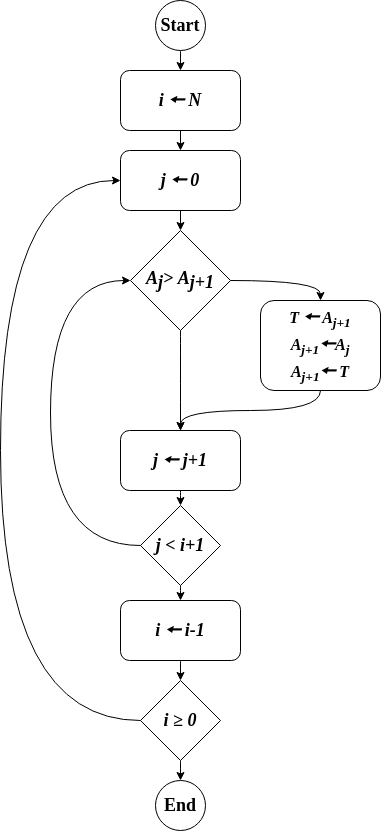
\includegraphics[width=6.5cm]{Chapter2/cfg.png}
  % \centering
  \caption{Control Flow Graph of bubblesort algorithm in Algorithm \ref{algo:bubble}}
  \label{fig:cfg}
\end{wrapfigure}

An execution processes a path (sequence) of instructions from an entry to any exit location of the program. For instance, consider Figure \ref{fig:cfg-heat} as a CFG illustrating the executed paths of 1000 trials of the program's execution. The numbers in the basic blocks indicate the number of times each basic block is visited. A path such as $A \rightarrow B \rightarrow E \rightarrow H \rightarrow I$ has been explored more than other execution paths. Basic block $D$ is visited occasionally and the edge $D \rightarrow I$ directly goes to the Exit, representing bugs in basic block $D$. These 1000 trials have discovered 9 seperable basic blocks, but it does not imply that there is no other basic blocks or edges revealed after more trials. Code coverage measures number of basic blocks which could be reached in an experiment of trials.

\begin{wrapfigure}{r}{6cm}
  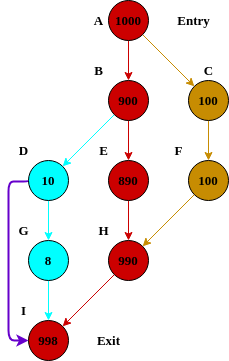
\includegraphics[width=5.5cm]{Chapter2/heatmap-cfg.png}
  \caption{CFG Heatmap \ref{algo:bubble}}
  \label{fig:cfg-heat}
\end{wrapfigure}

The vulnerabilities arise after target program executes with a triggering input. Miller introduced fuzz testing to examine the vulnerabilities of a collection of Unix utilities \cite{miller1990empirical}. The results showed that a random fuzzing on different versions of the utilities could discover bugs in 28\% of the targets. The automation in testing programs helps the researchers with validating the reliability of a program. The early fuzzers mimic a procedure of searching for the bugs by starting with \textit{identification} of the target program and its inputs. Next, the fuzzing loop initiates, and the program is run with fuzzed inputs as long as the fuzz testing is not terminated. Figure \ref{fig:fuzz_phases} depicts the fuzz testing procedure defined by Sutton et al. \cite{sutton2007fuzzing}. Based on the definitions, a standard fuzzer consists of:

\begin{itemize}
    \item Target identification
    \item Inputs identification
    \item Fuzzed data generation
    \item Execution of target with fuzzed data
    \item Exceptions monitoring
    \item Exploitability determination
\end{itemize}

\textbf{Target} is a software or a combination of executables and hardware \cite{song2019periscope}. A targeted software is any program that a machine can execute. 
Fuzzer needs to know the command for executing the target program and the inputs (arguments) of the program. \textbf{Inputs} are a set of environmental variables, file formats, and any other parameters that affect the execution. The initial seeds of the inputs can guide the fuzzer for finding more complex test cases, yet, it is not mandatory to provide seeds, and a fuzzer can generate valid inputs \textit{out of thin air} \cite{out_of_thin_air}. After the initial setup, the \textbf{fuzzing loop} begins iterating. In each iteration the fuzzer \textbf{executes} the target with the \textbf{provided test cases}. Fuzzer then looks for any exceptions returning from the executions and considers the executed input responsible for causing a \textbf{vulnerability}. The vulnerability can then be analyzed for \textbf{exploitability} in the last stage. An exploitable vulnerability can compromise the system and initiate an anomaly.

\begin{figure}[!b]
  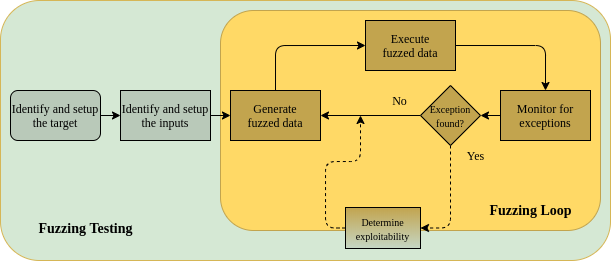
\includegraphics[width=\textwidth]{Chapter2/FuzzingPhases.png}
  \centering
  \caption{Fuzzing phases. Inspired by the definition of Sutton et al. \cite{sutton2007fuzzing}}
  \label{fig:fuzz_phases}
\end{figure}

The categories for fuzzers with different \textbf{program awareness} and different \textbf{techniques for fuzzing} the inputs help the community find different applications of the fuzzers for discovering more vulnerabilities. For instance, a developer uses a whitebox fuzzer to assess the immunity of the program (source-code accessible) against malicious activities. On the other hand, an attacker may use a blackbox fuzzer to attack a remote program blindly. A researcher may use a coverage-based fuzzer to consider the execution paths as a variable to reach more regions of the code and detect more crashes; hence, another researcher may use a performance fuzzer to reveal the test cases causing performance issues. 

\subsection{Program awareness}

% It must be explained in more details that these colorful categories are not accurate. 

The \textit{colorful} representation of fuzzers depends on the amount of information collected from a symbolic/concrete execution. A blackbox fuzzer does not gather any information from the execution. In contrast, whitebox fuzzers have all the required access to the program's source code, and greybox fuzzing covers the gray area between the mentioned types.

% Executes a lot - Easily scaled - No program awareness
% Shallow bugs
% Blackbox fuzzer
\subsubsection{Blackbox fuzzing}

Blackbox fuzz testing is a general method of testing an application without struggling with the analysis of the program itself. The target of an analysis executes after calling the proper API's, and the errors are expected to occur in the procedure of trying various inputs. Blackbox fuzzing is an effective technique though its simplicity \cite{woo2013scheduling}.

The introduced fuzzer by Miller \cite{miller1990empirical} was of the very first naive blackbox fuzzers. It runs the fuzzing for different lengths of inputs for each target (of the total 88 Unix utilities) and expects a \textbf{crash}, \textbf{hang}, or a \textbf{succeed} after the execution of the program. Each input is then fuzzed with a random mutation to generate new test cases. One of the \textbf{downsides} of blackbox fuzzing is that the program may face branches with \textit{magic values}, constraining the variables to a specific set of values; for instance, as shown in Listing \ref{lst:magic}, the chance of satisfying the equation $\texttt{magic\_string=="M4G!C"}$ and taking the \texttt{succeed()} path is almost zero. In \cite{banks2006snooze} and \cite{gascon2015pulsar} a set of network protocols are fuzzed in a blackbox manner, but as the target is specified, the performance is enhanced drastically. Any application on the web may be considered a blackboxed program as well, so as \cite{doupe2012enemy} and \cite{duchene2012xss} have targeted web applications and found ways to attack some the websites, looking for different vulnerabilities, such as XSS.

\begin{lstlisting}[language=C++,style=CodeStyle,caption=Magic Value: \texttt{M4G!C} is a magic value,label={lst:magic}]
  string magic_string = random_string();
  if(magic_string == "M4G!C")
      return succeed();
  else
      return failed();
\end{lstlisting}

A blackbox fuzzer is unaware of the program's structure and cannot monitor it's execution. The \textbf{benefit} of using a blackbox fuzzer is the speed of test case generation; the genuine compiled target program is being tested and the fuzzer does not put an effort on processing the inputs and executions. In addition, a blackbox fuzzer is featured to target external programs by using the standard interfaces of those programs. For instance, IoTFuzzer \cite{chen2018iotfuzzer} is an Internet of Things (IOT) blackbox fuzzer, \say{which aims at finding memory corruption vulnerabilities in IoT devices without access to their firmware images.} 
In a recent research by Mansur et al. \cite{mansur2020detecting}, they introduce a blackbox fuzzing method for detecting bugs in Satisfiability Modulo Theories (SMT) problems. As a result, blackbox fuzzing suggests a general solution in diverse domains. On the other hand, one of \textbf{drawbacks} of using blackbox fuzzing is that it finds \textit{shallow} bugs. A shallow vulnerability is an error that appears in the early discovered basic blocks in the CFG of the program. The reason behind this disadvantage is that blackbox fuzzing is \textbf{blind} in understanding the execution, and cannot analyze the CFG.

% Whitebox fuzzers

\subsubsection{Whitebox fuzzing}
% !        Rewrite this  |
% TODO     Rewrite this  V
Whitebox fuzzing works with the source code of the target. The knowledge of the program's logic helps the fuzzing procedure guided by satisfying the conditions resulting in new branches. Symbolic execution \cite{king1976symbolic} is a common whitebox fuzzing strategy that analyzes the source code and runs the program symbolically; the variables and inputs are replaced by symbols that the solution specifies the domain of the content inputs. Whitebox fuzzing leverages on symbolic executions for generating inputs that increase code coverage by discovering new branches after conditional instructions. This method helps the fuzzer detect deep bugs faster due to the powerful constraint solvers \cite{godefroid2008automated}. Despite the symbolic execution theoritically can solve the conditional branching, this technique suffers from \textit{path explosion} problem. For instance, in Figure \ref{fig:pathx} a sample section of a program containing a \texttt{loop} and an \texttt{if} statement within the loop. Figure \ref{fig:pathx3} shows the tree of the actions taken until the program reaches the basix block $X$. Solving the current loop requires an exponentially growing number of paths that the fuzzer needs to visit. Whitebox fuzzing is not very practical in the industry as it is very expensive (time-consuming / resource-consuming) and requires the source code, which may not be available for testers.

\begin{figure}[!b]
  \begin{adjustbox}{center,max width=1.3\textwidth}
      \begin{subfigure}[t]{0.30\textwidth}
          \centering
          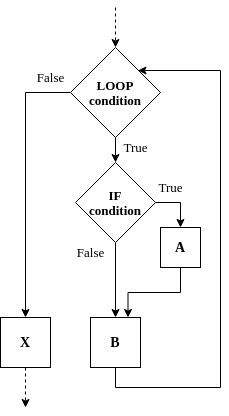
\includegraphics[width=\textwidth]{Chapter2/path-explosion.png}
          \vspace*{-5mm}
          \caption{Path explosion}
          \label{fig:pathx}
          \vspace*{5mm}
      \end{subfigure}
      ~
      \begin{subfigure}[b]{0.80\textwidth}
          \centering
          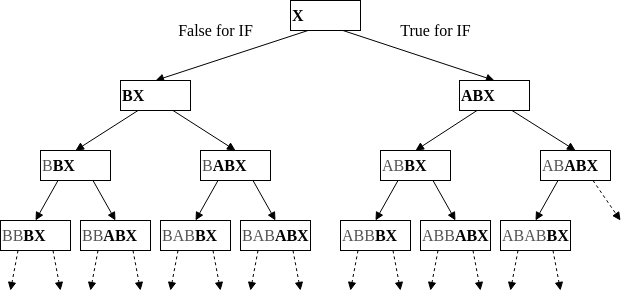
\includegraphics[width=\textwidth]{Chapter2/path-explosion-tree.png}
          \vspace*{-5mm}
          \caption{Path explosion tree}
          \label{fig:pathx3}
          \vspace*{5mm}
      \end{subfigure}
  \end{adjustbox}
  \caption{Path explosion example}
  \label{fig:path}
\end{figure}

SAGE \cite{godefroid2012sage}, a whitebox fuzzer, was developed as an alternative to blackbox fuzzing to cover the lacks of blackbox fuzzers \cite{cadar2011symbolic}. It can also use dynamic and \textit{concolic execution} \cite{stephens2016driller} and use taint analysis to locate the regions of seed files influencing values used by the program \cite{ganesh2009taint}. Concolic execution is an effective combination of symbolic execution and concrete (dynamic) executions; in a dynamic execution the fuzzer executes the program and analyzes the run.Godefroid et al. \cite{godefroid2008grammar} have also introduced a whitebox fuzzer that investigates the grammar for parsing the input files without any prior knowledge.

\subsubsection{Greybox fuzzing}

Greybox fuzzing resides between whitebox and blackbox fuzzing, as it has partial knowledge (awareness) about the internals of the target program. A \textbf{concrete execution} of a program represents a reproducible procedure that is executed that can be monitored for its behavior detection.

\subsection{Generation of inputs}

A fuzzer can check the code coverage of the test cases to detect new inputs with new execution behavior. For a coverage-based fuzzing, the corpus of inputs extends as the fuzzer finds new execution-paths. A performance fuzzer guides the fuzz testing to detect more resource-exhaustive procedures, and the usage of specific resources is more preferable than the code coverage.

\subsubsection{Coverage-based fuzzing}

Coverage-based fuzzing is a technique for fuzz testing that instruments the target without analyzing the logic of the program. In a greybox and whitebox coverage-based fuzzing, the instrumentation detects the different paths of the executions \cite{liang2018fuzzing}. AFL instruments the program with only the coverage information (section \nameref{sec:2-afl}).

The instrumentation can collect execution's data such as data coverage, statement coverage, block coverage, decision coverage, and path coverage \cite{yang2009survey}. Bohme et al. \cite{bohme2017coverage} introduced a coverage-based greybox fuzzer that extends AFL and benefits from the Markov Chain model. The fuzzer calculates the \textbf{energy} of the inputs based on the potency of a path for the discovery of new paths.

In another article by Bohme et al. \cite{bohme2017directed}, they introduce their directed fuzzing by the idea of checking the code coverage for providing inputs that guide the program execution toward some targeted locations. Some of the applications of such a fuzzing approach are patch testing and crash reproduction, which has different use cases compared to a non-directed coverage-based fuzzers.

\subsubsection{Performance fuzzing}

The \textbf{types} of vulnerabilities that a fuzzer is involved with may be different from other fuzzers. For example, AFL looks for crashes or hangs by selecting and mutating the inputs, and at the same time, it considers the code coverage, size of the inputs, and each execution time of the target program. PerfFuzz \cite{lemieux2018perffuzz} is a greybox fuzzer based on AFL, which aims to generate inputs for executions with higher \textbf{execution time} while using most of the features of AFL in code exploration. PerfFuzz counts how many times each of the edges of the control flow graph (CFG) is executed. Using SlowFuzz \cite{petsios2017slowfuzz}, Petsios et al. lets the fuzzer use any execution features for detecting the worst-case scenarios (inputs) for the selected features. In another project based on AFL, Memlock \cite{wen2020memlock} investigates memory exhaustion by calculating the maximum runtime memory required during executions. A disadvantage in previous works in performance is that the development of the fuzzer for considering different instructions is cumbersome.

\vspace{1.5\baselineskip}
